\section{Problem B}
\textit{Use the Matlab random number generator to generate several (how many is 'several'?) realizations of the channel (one realization = one set of complex values, each one corresponding to the complex tap gain of the taps). Store these values. Calculate the average power delay profile based on these realization, and from that find the delay spread. Is it in good agreement with the result from (A)?}\\
 
In order to generate the complex impulse response each tap gain of the power has to be multiplied whit the random complex number that has been created using \textit{randn} function in Matlab. After that 1000 realizations are run. The impulse response is Rayleigh distributed.

\code{language=Matlab,caption = Impulse Response Calculation,label=cl:imp_resp_code,linerange={36-40},firstnumber=36}{code/mm1/mm1_pretty_solution_pretty_coments_Labels_and_DB.m}

Than, the calculation of the average power delay profile is made by doing the mean of the absolute value of \textit{h}. This is shown in the \figref{fig:Impulse_Response} :

\begin{figure}
\centering
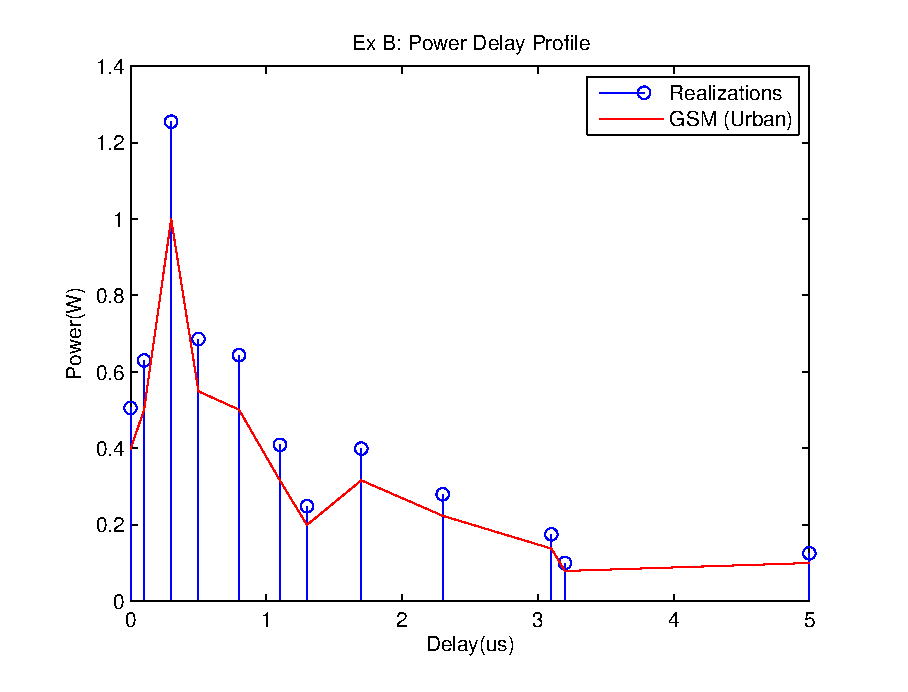
\includegraphics[width=9cm]{PDP.eps}
\caption{Impulse Response and PDP}\label{fig:Impulse_Response}
\end{figure}